\documentclass[12pt, a4paper]{report}

% Packages :

\usepackage[french]{babel}
\usepackage[utf8]{inputenc}
\usepackage[T1]{fontenc}
\usepackage[pdftex, pdfauthor={Bacomathiques}]{hyperref}
\usepackage{sectsty}
\usepackage[explicit]{titlesec}
\usepackage{xcolor}
\usepackage{amsmath}
\usepackage{amssymb}
\usepackage{amsthm}
\usepackage{fourier}
\usepackage{titlesec}
\usepackage{fancyhdr}
\usepackage{catchfilebetweentags}
\usepackage[french, capitalise, noabbrev]{cleveref}
\usepackage[fit, breakall]{truncate}
\usepackage[margin=3cm]{geometry}
\usepackage{tocloft}
\usepackage{tikz}
\usepackage{tocloft}
\usepackage{microtype}
\usepackage{listings}
\usepackage{tabularx}
\usepackage{calc}
\usepackage[export]{adjustbox}
\usepackage[most]{tcolorbox}
\usepackage{standalone}
\usepackage{xlop}
\usepackage{etoolbox}
\usepackage{environ}

\usetikzlibrary{arrows.meta}
\usetikzlibrary{trees}

% Paramètres :

\author{Bacomathiques}
\definecolor{graphe}{HTML}{93c9ff}
\setcounter{MaxMatrixCols}{12}
\setlength{\parindent}{0pt}
\setlength{\fboxsep}{0pt}
%\pdfsuppresswarningpagegroup=1

% Code :

\lstdefinestyle{style}{
	backgroundcolor=\color{white},
	commentstyle=\em\color[HTML]{999988},
	keywordstyle=\bfseries,
	identifierstyle=\normalfont,
	stringstyle=\color[rgb]{0.87, 0.07, 0.27},
	basicstyle=\ttfamily\color{black},
	breakatwhitespace=false,
	breaklines=true,
	captionpos=b,
	keepspaces=true,
	numbers=left,
	numbersep=5pt,
	showspaces=false,
	showstringspaces=false,
	showtabs=false,
	tabsize=2,
	numbers=none
}

\lstset{style=style}
\lstset{
	literate=
	{á}{{\'a}}1
	{à}{{\`a}}1
	{ã}{{\~a}}1
	{é}{{\'e}}1
	{ê}{{\^e}}1
	{í}{{\'i}}1
	{ó}{{\'o}}1
	{õ}{{\~o}}1
	{ú}{{\'u}}1
	{ü}{{\"u}}1
	{ç}{{\c{c}}}1
}

\lstset{
	framextopmargin=10pt,
	framexrightmargin=10pt,
	framexbottommargin=10pt,
	framexleftmargin=10pt,
	xleftmargin=10pt,
	xrightmargin=10pt,
}

% Couleurs :

\definecolor{title}{HTML}{912c21}
\definecolor{section}{HTML}{1c567d}
\definecolor{subsection}{HTML}{2980b9}

\definecolor{rule}{HTML}{c4c4c4}

\definecolor{formula}{HTML}{ebf3fb}
\definecolor{formula-left}{HTML}{3583d6}

\definecolor{tip}{HTML}{dcf3d8}
\definecolor{tip-left}{HTML}{26a65b}

\definecolor{demonstration}{HTML}{fff8de}
\definecolor{demonstration-left}{HTML}{f1c40f}

\definecolor{exercise}{HTML}{e0f2f1}
\definecolor{exercise-left}{HTML}{009688}

\definecolor{correction}{HTML}{e0f7fa}
\definecolor{correction-left}{HTML}{00bcd4}

\definecolor{toc}{HTML}{fceae9}
\definecolor{toc-left}{HTML}{e74c3c}
\definecolor{toc-dark}{HTML}{87281f}

% Titres :

\renewcommand{\thesection}{\Roman{section} - }
\renewcommand{\thesubsection}{\arabic{subsection}. }

\newcommand{\sectionstyle}{\normalfont\LARGE\bfseries\color{section}}
\titleformat{\section}{\sectionstyle}{\thesection #1}{0pt}{}
\titleformat{name=\section, numberless}{\sectionstyle}{#1}{0pt}{}

\newcommand{\subsectionstyle}{\normalfont\Large\bfseries\color{subsection}}
\titleformat{\subsection}{\subsectionstyle}{\thesubsection #1}{0pt}{}
\titleformat{name=\subsection, numberless}{\subsectionstyle}{#1}{0pt}{}

\titlelabel{\thetitle\ }

% Table des matières :

\addto\captionsfrench{\renewcommand\contentsname{}}
\renewcommand{\cftsecpagefont}{\color{toc-dark}}
\renewcommand{\cftsubsecpagefont}{\color{toc-dark}}
\renewcommand{\cftsecleader}{\cftdotfill{\cftdotsep}}
\renewcommand{\cftsecfont}{\bfseries}
\renewcommand{\cftsecpagefont}{\bfseries\color{toc-dark}}
\setlength{\cftbeforetoctitleskip}{0pt}
\setlength{\cftaftertoctitleskip}{0pt}
\setlength{\cftsecindent}{0pt}
\setlength{\cftsubsecindent}{20pt}
\setlength{\cftsubsecnumwidth}{20pt}

% Commandes :

\newcommand{\newpar}{\\[\medskipamount]}
\newcommand{\lesson}[3]{%
	\newcommand{\level}{#1}%
	\newcommand{\id}{#2}%
	\hypersetup{pdftitle={#3}}
	\begin{center}%
		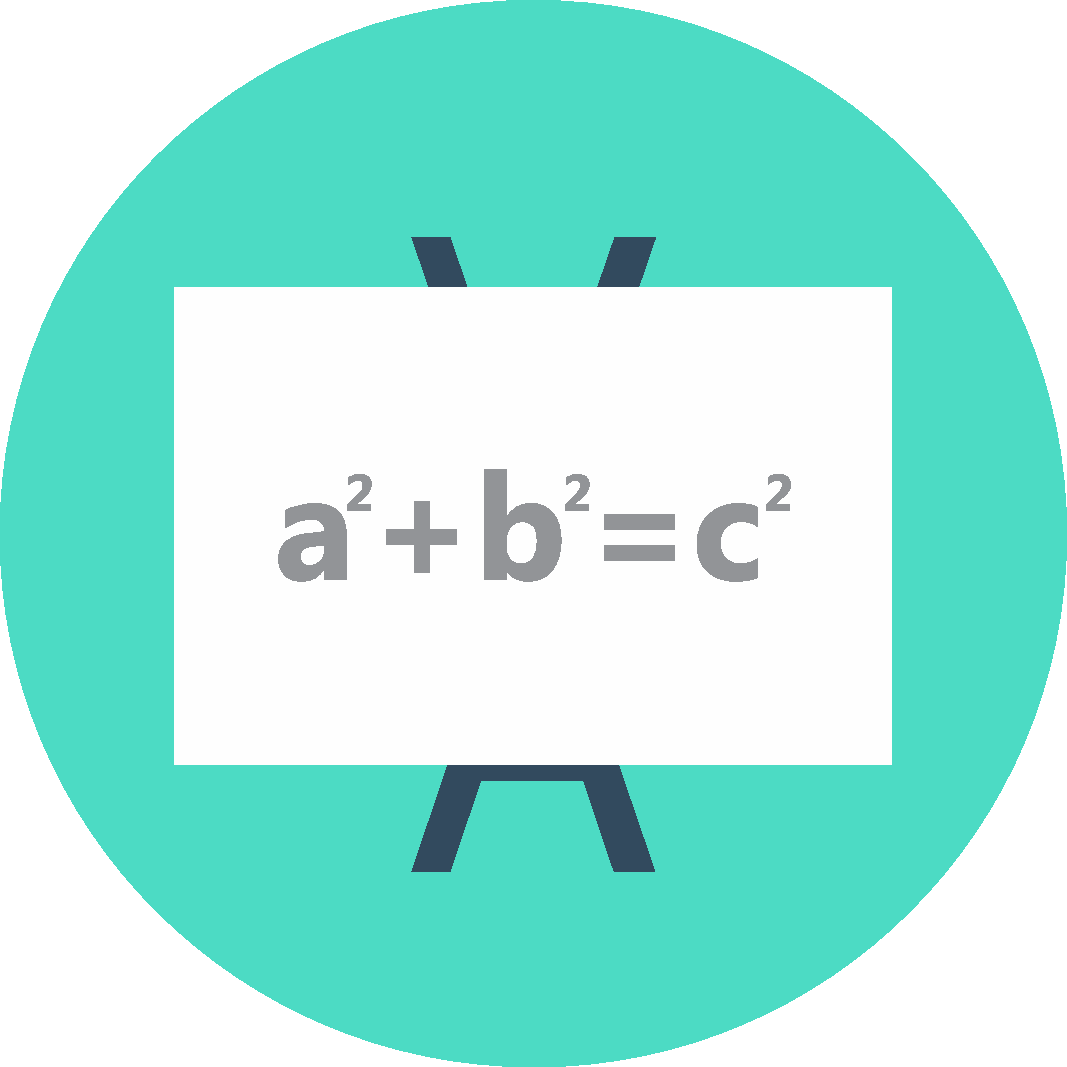
\includegraphics[width=150px]{\imagespath/bacomathiques}%
		
		\vspace{30pt}%
		{\Huge\color{title} #3}%
		
		\vspace{10pt}%
		{Bacomathiques --- \href{https://bacomathiqu.es/cours/#1/#2}{\color{section} https://bacomathiqu.es}}%
		
		\vspace{20pt}%
	\end{center}%
	\begin{toc}
		\tableofcontents%
	\end{toc}
	\thispagestyle{empty}%
	\newpage%
	\setcounter{page}{1}%
}
\newcommand{\imagespath}{../../images}
\newcommand{\lessonimagespath}{\imagespath/lessons/\level/\id/}
\newcommand{\includelatexpicture}[2][\textwidth - 100pt]{%
	\begin{center}%
		\resizebox{#1}{!}{%
			\input{\lessonimagespath#2}%
		}%
	\end{center}%
	\medskip%
}
\newcommand{\includeimage}[1]{%
	\begin{center}%
		\includegraphics{\lessonimagespath#1}%
	\end{center}%
	\medskip%
}
\newcommand{\includerepresentation}[1]{%
	\begin{center}%
		\setlength{\fboxrule}{0.5pt}%
		\href{https://www.geogebra.org/m/#1}{\includegraphics[width=\textwidth-1pt,fbox]{\lessonimagespath#1}}%
	\end{center}%
}
\newcommand{\floor}[1]{\lfloor #1 \rfloor}

\makeatletter
\newcommand\inputcontent{\@ifstar{\inputcontent@star}{\inputcontent@nostar}}
\newcommand{\inputcontent@star}[1]{%
	\ExecuteMetaData[#1]{content}%
}
\newcommand{\inputcontent@nostar}[1]{%
	\newpage%
	\inputcontent@star{#1}%
}
\makeatother

\let\oldsection\section
\renewcommand\section{\clearpage\oldsection}
\newcommand{\contentwidth}[1][medium]{}

% En-têtes :

\pagestyle{fancy}

\renewcommand{\sectionmark}[1]{\markboth{\thesection \ #1}{}}

\fancyhead[R]{\truncate{0.23\textwidth}{\color{title}\thepage}}
\fancyhead[L]{\truncate{0.73\textwidth}{\color{title}\leftmark}}
\fancyfoot[C]{\scriptsize \href{https://bacomathiqu.es/cours/\level/\id}{\texttt{bacomathiqu.es}}}

\makeatletter
\patchcmd{\f@nch@head}{\rlap}{\color{rule}\rlap}{}{}
\patchcmd{\headrule}{\hrule}{\color{rule}\hrule}{}{}
\makeatother

% Environnements :

\newenvironment{nosummary}{}{}
\newcommand{\tcolorboxtitle}[2]{\setlength{\fboxsep}{2.5pt}\hspace{-10pt}\colorbox{#1-left}{\hspace{8pt}\MakeUppercase{#2} \hspace{2pt} \includegraphics[height=0.8em]{\imagespath/bubbles/#1}\hspace{5pt}}}
\newcommand{\tcolorboxsubtitle}[2]{\ifstrempty{#2}{}{\textcolor{#1-left}{\large#2}\\[\medskipamount]}}
\tcbset{
	frame hidden,
	boxrule=0pt,
	boxsep=0pt,
	enlarge bottom by=8.5pt,
	enhanced jigsaw,
	boxed title style={sharp corners,boxrule=0pt,coltitle={white},titlerule=0pt},
	fonttitle=\fontsize{6pt}{6pt}\bfseries\boldmath,
	top=10pt,
	right=10pt,
	bottom=10pt,
	left=10pt,
	arc=0pt,
	outer arc=0pt,
}
\newtcolorbox{toc}[1][]{
	colback=toc,
	borderline west={3pt}{0pt}{toc-left},
	title=\tcolorboxtitle{toc}{Table des matières},
	colbacktitle=toc,
	before upper={\tcolorboxsubtitle{toc}{#1}}
}
\newtcolorbox{formula}[1][]{
	colback=formula,
	borderline west={3pt}{0pt}{formula-left},
	title=\tcolorboxtitle{formula}{À retenir},
	colbacktitle=formula,
	before upper={\tcolorboxsubtitle{formula}{#1}}
}
\newtcolorbox{tip}[1][]{
	colback=tip,
	borderline west={3pt}{0pt}{tip-left},
	title=\tcolorboxtitle{tip}{À lire},
	colbacktitle=tip,
	before upper={\tcolorboxsubtitle{tip}{#1}}
}
\newtcolorbox{demonstration}[1][]{
	colback=demonstration,
	borderline west={3pt}{0pt}{demonstration-left},
	title=\tcolorboxtitle{demonstration}{Démonstration},
	colbacktitle=demonstration,
	before upper={\tcolorboxsubtitle{demonstration}{#1}}
}

\NewEnviron{whitetabularx}[1]{%
	\renewcommand{\arraystretch}{2.5}
	\colorbox{white}{%
		\begin{tabularx}{\textwidth}{#1}%
			\BODY%
		\end{tabularx}%
	}%
}

% Longueurs :

\newlength{\espacetitreliste}
\setlength{\espacetitreliste}{-16pt}
\newcommand{\entretitreetliste}{\vspace{\espacetitreliste}}

\begin{document}
	%<*content>
	\lesson{terminale}{primitives-equations-differentielles}{Chapitre VI – Primitives et équations différentielles}

	\section{Primitives de fonctions continues}

	\subsection{Définition}

	\begin{formula}[Définition]
		Soit $f$ une fonction définie et continue sur un intervalle $I$. On appelle \textbf{primitive} de $f$, toute fonction $F$ définie sur $I$ et qui vérifie pour tout $x \in I$ : $F'(x) = f(x)$.
	\end{formula}

	\begin{tip}[Note]
		Une primitive est toujours définie à une constante près.
		\newpar
		En effet. On considère la fonction $f$ définie pour tout $x \in \mathbb{R}$ par $f(x) = 2x$. Alors, $F_{1} : x \mapsto x^2 + 1$ est une primitive de la fonction $f$ (car pour tout $x$, $F'(x) = 2x = f(x)$).
		\newpar
		Mais $F_{1}$ \textbf{n'est pas la seule primitive} de $f$ ! On peut citer par exemple $F_{2} : x \mapsto x^2 + 10$ et $F_{3} : x \mapsto x^2 + 3$ qui sont également des primitives de $f$.
		\newpar
		C'est pour cette raison que l'on dit que les primitives sont définies à une constante près (lorsque l'on dérive, la constante devient nulle).
	\end{tip}

	Ainsi, toute \textbf{fonction continue} sur un intervalle admet \textbf{une infinité de primitives} d'une forme particulière sur cet intervalle. Plus formellement :

	\begin{formula}[Infinité de primitives]
		Une fonction continue $f$ sur un intervalle $I$ admet une infinité de primitives sur $I$ de la forme $x \mapsto F_0(x) + c$ avec $c \in \mathbb{R}$ (où $F_0$ est une primitive de $f$).
	\end{formula}

	\begin{demonstration}[Infinité de primitives]
		Soit $F$ une autre primitive de $f$ sur $I$. On a pour tout $x \in I$ :
		\newpar
		$(F - F_0)'(x) = F'(x) - F_0'(x) = f(x) - f(x) = 0$ (car $F_0$ et $F$ sont deux primitives de $f$).
		\newpar
		Donc il existe une constante réelle $c$ telle que $F - F_0 = c$. D'où pour tout $x \in I$, $F(x) = F_0(x) + c$ : ce qu'il fallait démontrer.
	\end{demonstration}

	\subsection{Primitive de fonctions usuelles}

	Le tableau suivant est à connaître (mais il peut être obtenu en prenant celui des dérivées usuelles à l'envers) :

	\begin{formula}
		Soit $\lambda$ une constante réelle.
		\newpar
		\begin{whitetabularx}{|X|X|X|}
			\hline
			\textbf{Fonction} & \textbf{Primitive} & \textbf{Domaine de définition de la primitive} \\
			\hline
			$\lambda$ & $\lambda x$ & $\mathbb{R}$ \\
			\hline
			$e^x$ & $e^x$ & $\mathbb{R}$ \\
			\hline
      $\displaystyle{\frac{1}{x}}$ & $\ln(x)$ & $\mathbb{R}^{*}_{+}$ \\
			\hline
			$\displaystyle{\frac{1}{\sqrt{x}}}$ & $2\sqrt{x}$ & $\mathbb{R}^{*}_{+}$ \\
			\hline
			$x^a$ avec $a \in \mathbb{R}$ et $a \neq -1$ & $\displaystyle{\frac{1}{a + 1} x^{a + 1}}$ & $\mathbb{R}^{*}_{+}$ \\
			\hline
			$\sin(x)$ & $-\cos(x)$ & $\mathbb{R}$ \\
			\hline
			$\cos(x)$ & $\sin(x)$ & $\mathbb{R}$ \\
			\hline
		\end{whitetabularx}
	\end{formula}

	\subsection{Opérations sur les primitives}

	Le tableau suivant est également à connaître (mais il peut être obtenu en prenant celui des dérivées usuelles à l'envers) :

	\begin{formula}
		Soit $u$ une fonction continue.
		\newpar
		\begin{whitetabularx}{|X|X|X|}
			\hline
			\textbf{Fonction} & \textbf{Primitive} & \textbf{Domaine de définition de la primitive} \\
			\hline
			$u'e^u$ & $e^u$ & En tout point où $u$ est définie. \\
			\hline
			$\displaystyle{\frac{u'}{u}}$ & $\ln(|u|)$ & En tout point où $u$ est définie et est non-nulle. On peut retirer la valeur absolue si $u$ est positive. \\
			\hline
			$\displaystyle{\frac{u'}{\sqrt{u}}}$ & $2\sqrt{u}$ & En tout point où $u$ est définie et est strictement positive. \\
			\hline
			$u' (u)^a$ avec $a \in \mathbb{R}$ et $a \neq -1$ & $\displaystyle{\frac{1}{a + 1} u^{a + 1}}$ & En tout point où $u$ est définie. \\
			\hline
			$u' \sin(u)$ & $-\cos(u)$ & En tout point où $u$ est définie. \\
			\hline
			$u' \cos(u)$ & $\sin(u)$ & En tout point où $u$ est définie. \\
			\hline
		\end{whitetabularx}
	\end{formula}

	\section{Équations différentielles}

	\subsection{Qu'est-ce-qu'une équation différentielle ?}

	Commençons cette partie par quelques définitions.

	\begin{formula}[Définition]
		\begin{itemize}
			\item Une \textbf{équation différentielle} est une égalité liant une fonction inconnue $y$ à ses dérivées successives ($y'$, $y''$, ...) contenant éventuellement d'autres fonctions connues.
			\item Une \textbf{solution} d'une équation différentielle est une fonction vérifiant l'égalité décrite précédemment.
		\end{itemize}
	\end{formula}

	\begin{tip}[Exemple]
		La fonction logarithme est une solution de l'équation différentielle $y' = \frac{1}{x}$.
		\newpar
		La fonction exponentielle est une solution de l'équation différentielle $y' = y$, mais aussi de l'équation différentielle $y'' = y$, etc.
	\end{tip}

	\subsection{Résolution d'équations différentielles de la forme $y'=ay$}

	Nous allons donner une formule permettant de résoudre des équations différentielles de la forme $y' = ay$.

	\begin{formula}[Formule]
		On pose $(E) : y'=ay$ (où $a$ est un réel). Alors l'ensemble des solutions de $(E)$ est l'ensemble des fonctions $x \mapsto c e^{ax}$ où $c \in \mathbb{R}$.
	\end{formula}

	\begin{demonstration}
		Vérifions tout d'abord que les fonctions $x \mapsto k e^{ax}$ sont solutions de $(E)$. Soit $c \in \mathbb{R}$, posons pour tout $x \in \mathbb{R}$, $y_c(x) = c e^{ax}$.
		\newpar
		Alors pour tout $x \in \mathbb{R}$, $y'_c(x) = ac e^{ax}$ et $ay_c(x) = ac e^{ax}$. Donc $y'_c = a y_c$ : $y_c$ est bien solution de $(E)$.
		\newpar
		Montrons que les fonctions $y_c$ sont les seules solutions de $(E)$. Soit $y$ une solution quelconque de $(E)$ sur $\mathbb{R}$. Pour tout $x \in \mathbb{R}$, on pose $z(x) = y(x) e^{-ax}$. En dérivant :
		\newpar
		$z'(x) = y'(x) e^{-ax} + y(x) (-ae^{-ax}) = e^{-ax}(y'(x) - ay(x))$
		\newpar
		De plus, comme $y$ est solution de $(E)$, on a $y' - ay = 0$, donc $z' = 0$.
		\newpar
		Ainsi, il existe une constante réelle $c$ telle que $z = c$. C'est-à-dire que pour tout $x \in \mathbb{R}$ :
		\newpar
		$c = y(x) e^{-ax} \iff y(x) = c e^{ax}$. Ce qui termine la preuve.
	\end{demonstration}

	\begin{formula}[Théorème]
		Pour tout réels $x_0$ et $y_0$, il existe une \textbf{unique} fonction $y$ solution de l'équation différentielle $(E)$ telle que $y(x_0) = y_0$.
	\end{formula}

	\begin{tip}[Exemple]
		Résolvons l'équation différentielle $(E) : y' - 5y = 0$ sous condition d'avoir $y(0) = 1$.
		\newpar
		Dans un premier temps, on écrit l'équation sous une meilleure forme : $y' - 5y = 0 \iff y' = 5y$. On a donc $a = 5$. Les solutions de l'équation $(E)$ sont les fonctions définies $x \mapsto c e^{5x}$ où $c \in \mathbb{R}$.
		\newpar
		Maintenant, il faut trouver la fonction $y$ qui vaut $1$ en $0$. Soit donc $y$ une telle solution de $(E)$. Alors :
		\newpar
		$y(0) = 1 \iff c e^{5 \times 0} = 1 \iff c = e^{-1}$. La solution recherchée est donc la fonction $y : x \mapsto e^{-1} e^{5x}$.
	\end{tip}

	\subsection{Résolution d'équations différentielles de la forme \texorpdfstring{$y'=ay+b$}{y'=ay+b}}

	Nous allons donner une formule permettant de résoudre des équations différentielles de la forme $y' = ay+b$.

	\begin{formula}[Formule]
		On pose $(E) : y'=ay+b$ (où $a$ est un réel non-nul et $b$ est un réel). Alors l'ensemble des solutions de $(E)$ est l'ensemble des fonctions $x \mapsto c e^{ax} - \frac{b}{a}$ où $c \in \mathbb{R}$.
	\end{formula}

	\begin{formula}[Théorème]
		Pour tout réels $x_0$ et $y_0$, il existe une \textbf{unique} fonction $y$ solution de l'équation différentielle $(E)$ telle que $y(x_0) = y_0$.
	\end{formula}

	\begin{tip}[Exemple]
		Résolvons l'équation différentielle $(E) : y'=2y-1$ sous condition d'avoir $y(1) = 0$.
		\newpar
		On a donc $a = 2$ et $b = -1$. Les solutions de l'équation $(E)$ sont les fonctions définies $x \mapsto c e^{2x} + \frac{1}{2}$ où $c \in \mathbb{R}$.
		\newpar
		Maintenant, il faut trouver la fonction $y$ qui vaut $0$ en $1$. Soit donc $y$ une telle solution de $(E)$. Alors :
		\newpar
		$y(1) =  0 \iff c e^{2 \times 1} + \frac{1}{2} = 0 \iff c = -\frac{1}{2e^2}$. La solution recherchée est donc la fonction $y : x \mapsto -\frac{e^{2x}}{2e^2} + \frac{1}{2}$.
	\end{tip}
	%</content>
\end{document}
